\newpage
\begin{center}
  \textbf{\large ПРИЛОЖЕНИЕ А}
\end{center}
\refstepcounter{chapter}
\addcontentsline{toc}{chapter}{ПРИЛОЖЕНИЕ А Параметры вариаций}

\label{sec:params}
\begin{table}[h]
  \caption{Параметры рандомизаций на задаче с отрытием шкафа}
  \label{res-Table3}
  \centering{
    \begin{tabular}{ | @{\hskip 5pt} p{5cm} @{\hskip 5pt} | @{\hskip 5pt} p{5cm} @{\hskip 5pt} | @{\hskip 5pt} p{5cm} @{\hskip 5pt} | }
      \hline
      Рандомизация & Описание & Параметры \\ \hline 
     Отсутствие рандомизаций & Исходная среда & -  \\ \hline
     \multicolumn{3}{|c|}{\textit{Визуальные параметры}} \\ \hline  
     Текстура ОМ & Рандомизированная текстура шкафа & $\mathrm{Uniform}(\mathcal{X}_{textures})$ \\ \hline
     Цвет ОМ & Рандомизированный цвет шкафа  & $\mathrm{Uniform}(0.0, 1.0)$  \\ \hline
     Текстура заднего плана & Рандомизированная текстура стен & $\mathrm{Uniform}(\mathcal{X}_{textures})$  \\ \hline
     Цвет заднего плана & Рандомизированный цвет стен & $\mathrm{Uniform}(0.0, 1.0)$ \\ \hline
     Цвет источника освещения & Рандомизированный цвет освещения & $\mathrm{Uniform}(0.0, 0.75)$ \\ \hline
     Отвлекающий объект & Рандомизированное положение отвлекающего объекта & $\mathrm{Uniform}(-0.05, 0.05)$ \\ \hline
     Смещение камеры & Рандомизированное положение камеры & $\mathrm{Uniform}(-0.005, 0.005)$  \\ \hline
      \multicolumn{3}{|c|}{\textit{Физические параметры}} \\ \hline  
       Масса объектов & Рандомизированная масса шкафа & $\mathrm{Uniform}(0.1, 4.1)$ \\ \hline 
       Трения объектов & Рандомизированные коэффициенты трения шкафа & $\mathrm{Uniform}(0.5, 1.5)$  \\ \hline
    \end{tabular}
  }
  
\end{table}

\begin{table}[h]
  \caption{Параметры рандомизаций на задаче взятия банки}
  \label{res-Table3}
  \centering{
    \begin{tabular}{ | @{\hskip 5pt} p{5cm} @{\hskip 5pt} | @{\hskip 5pt} p{5cm} @{\hskip 5pt} | @{\hskip 5pt} p{5cm} @{\hskip 5pt} | }
      \hline
      Рандомизация & Описание & Параметры \\ \hline 
     Отсутствие рандомизаций & Исходная среда & -  \\ \hline
     \multicolumn{3}{|c|}{\textit{Визуальные параметры}} \\ \hline  
     Текстура ОМ & Рандомизированная текстура банки & $\mathrm{Uniform}(\mathcal{C}_{textures})$ \\ \hline
     Цвет ОМ & Рандомизированный цвета банки  & $\mathrm{Uniform}(0.5, 1.0)$  \\ \hline
     Текстура заднего плана & Рандомизированная текстура стола & $\mathrm{Uniform}(\mathcal{X}_{textures})$  \\ \hline
     Цвет заднего плана & Рандомизированный цвет стола & $\mathrm{Uniform}(0.5, 1.0)$ \\ \hline
     Цвет источника освещения & Рандомизированный цвет освещения & $\mathrm{Uniform}(0.5, 1.0)$ \\ \hline
     Отвлекающий объект & Рандомизированное положение отвлекающего объекта & $\mathrm{Uniform}(-0.05, 0.05)$ \\ \hline
     Смещение камеры & Рандомизированное положение камеры & $\mathrm{Uniform}(-0.03, 0.03)$  \\ \hline
      \multicolumn{3}{|c|}{\textit{Физические параметры}} \\ \hline  
       Масса объектов & Рандомизированная масса банки & $\mathrm{Uniform}(0.1, 1.9)$ \\ \hline 
       Трения объектов & Рандомизированные коэффициенты трения банки & $\mathrm{Uniform}(0.5, 1.5)$  \\ \hline
    \end{tabular}
  }
  
\end{table}

Множество $\mathcal{X}_{textures}$ взято из коллекции текстур дерева из Isaac Lab. Множество $\mathcal{C}_{textures}$ взято из открытой коллекции текстур банок. 

\clearpage
\newpage
\begin{center}
  \textbf{\large ПРИЛОЖЕНИЕ Б}
\end{center}
\refstepcounter{chapter}
\addcontentsline{toc}{chapter}{ПРИЛОЖЕНИЕ Б Примеры рандомизаций}
\label{sec:randomization}

\begin{figure}[h]
  \begin{center}
      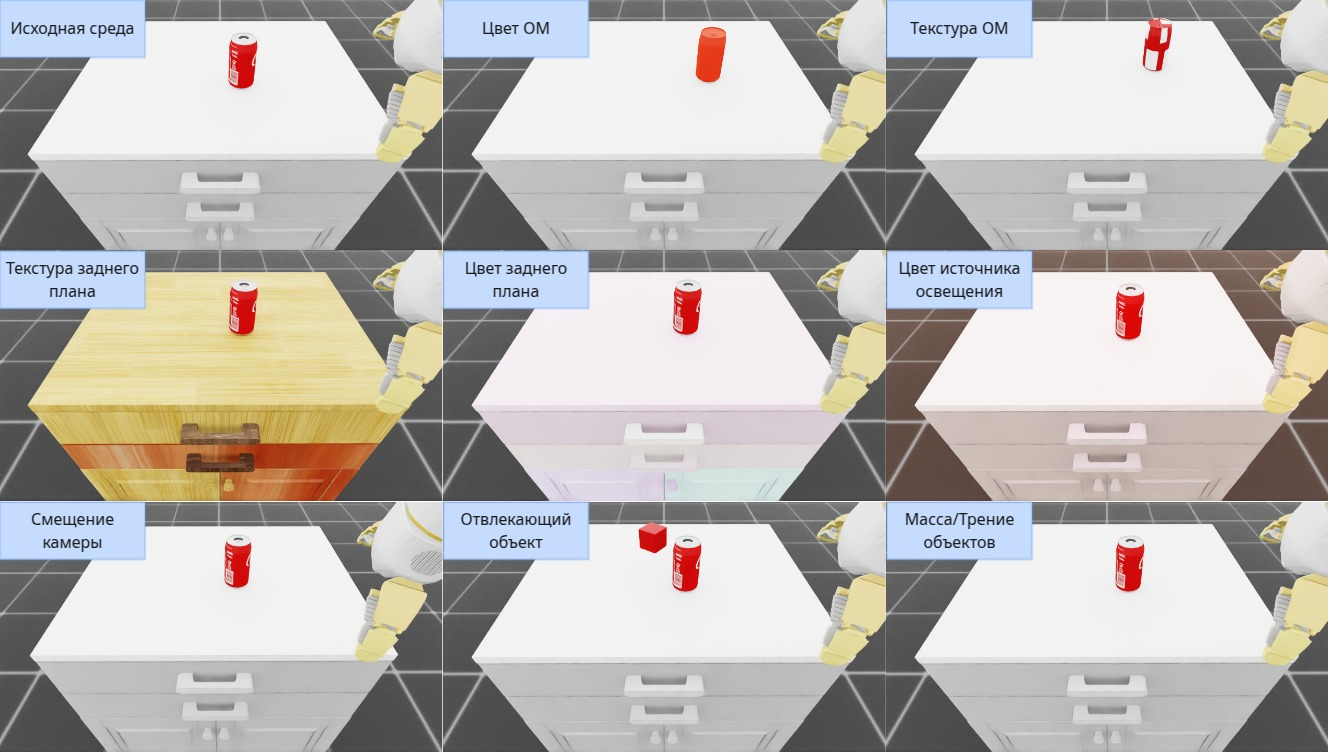
\includegraphics[width=\textwidth]{images/Randomizations.jpg}
  \caption{Пример рандомизаций для задачи взятия банки}
  \end{center}
\end{figure}

\clearpage
\newpage
\begin{center}
  \textbf{\large ПРИЛОЖЕНИЕ В}
\end{center}
\refstepcounter{chapter}
\addcontentsline{toc}{chapter}{ПРИЛОЖЕНИЕ В Программная реализация метода}
\label{sec:program}

\begin{figure}[h]
  \begin{center}
      
\includegraphics[width=0.8\textwidth]{images/463b52fd-5ec1-41eb-a46c-899e347383db.png}
  \caption{QR-код с ссылкой на репозиторий https://github.com/StriderOne/EnvForge.git, содержащий программную реализацию метода}
  \label{fig:arch}
  \end{center}
\end{figure}